\documentclass[a4paper]{article}

\usepackage[english]{babel}
\usepackage[utf8]{inputenc}
\usepackage{amsmath} % THE mathematic package
\usepackage{amsfonts} % Some math fonts
\usepackage{mathrsfs}
\usepackage{stmaryrd} % For the llbracket
\usepackage[retainorgcmds]{IEEEtrantools} %array environment
\usepackage[lined,algonl,boxed]{algorithm2e}
%\usepackage{algpseudocode}
\usepackage{graphicx}
\usepackage[colorinlistoftodos]{todonotes} % For comments \todo{Big boobs!!}
\usepackage[colorlinks=true,linkcolor=blue]{hyperref} % Hyperlinks within the document, \url, href, tableofcontents,ect.

\title{Notes on 3D PSF microscopy}

\author{James Bond, Goldorak}

\date{\today}

\begin{document}
\maketitle
\begin{abstract}
This paper detailsssss the implementation of the 3D PSF modeled after a parametrized pupil function of wide field fluorescence microscopy (WFFM). The goal is to connect 
for a better comprehension of the code.
\end{abstract}
\tableofcontents

%%%%%%%%%%%%%%%%%%%%%%%%%%%%%%%%%%%%%%%%%%%%%%%%%%%%%%%%%%%%%%%%%%%%
%INTRODUCTION
%%%%%%%%%%%%%%%%%%%%%%%%%%%%%%%%%%%%%%%%%%%%%%%%%%%%%%%%%%%%%%%%%%%%
\section{Introduction}

What, who, where, when?
This paper details the implementation of the 3D point spread function modeled after a parametrized pupil function of wide field fluorescence microscopy (WFFM)\cite{3DBlind}.
The main purpose of this document is to provide basic understanding of the algorithm and support for the furture project work. The connection between equation and code will be detailed.
First coded in Yorick and C, algorithms are now coded in Java for a better portability.
A review of definitions are explained then some

%%%%%%%%%%%%%%%%%%%%%%%%%%%%%%%%%%%%%%%%%%%%%%%%%%%%%%%%%%%%%%%%%%%%
%DEFINITIONS
%%%%%%%%%%%%%%%%%%%%%%%%%%%%%%%%%%%%%%%%%%%%%%%%%%%%%%%%%%%%%%%%%%%%
\section{Definitions}
\todo[inline, color=green!40]{Expliquer les notations, la taille. L'image aux pixel i,j;donné leurs amplitude $\in \mathbb{N}$ ou plutot $\in [0,N_x]$, pareil pour $z$}

%---------------Notations----------------
\subsection{Convention, notation}
\begin{itemize}
\item $(i,j)$ : pixel position at $i$-th row and $j$-th column with $i \in \llbracket 0, m-1\rrbracket$, $j \in \llbracket 0, n-1\rrbracket$ for a $m$ rows and $n$ columns matrix image.
\item $(x,y,z)$ : cartesian coordinate.
\end{itemize}

%---------------PSF----------------
\subsection{PSF}
Based on Born and Wolf model\cite{born}, the point spread function $h$ at the depth $z$ is described as the square modulus of the Fourier transform of the pupil function : 
\begin{equation}
h_{i,j}(z) = |\hat{A}_{i,j}(z)|^2
\end{equation}
with $i,j$ the pixel position, $\hat{A} = a$ the discret Fourier transform of the pupil function $A$.

%---------------Pupil function----------------
\subsection{Pupil function $a$}
\begin{equation}
A_{i,j}(z) = \rho_{i,j} e^{\iota\Phi_{i,j}(z)} = \rho_{i,j} \exp( \iota(\varphi_{i,j} + 2\pi(d \omega_{i,j} + z \psi_{i,j})))
\end{equation}

\begin{itemize}
\item $\iota$ the complex number.
\item $\displaystyle{\rho_{i,j} = \sum_n \beta_n Z_{i,j}^n}$ the pupil modulus with $\beta_n$ the Zernike coefficients and $Z_{i,j}^n$ the n-th Zernike polynomial (see~\ref{Z}) for pixel $(i,j)$.
\item $\Phi_{i,j}$ the argument of the pupil.
\item $\displaystyle{\varphi_{i,j} = \sum_n \alpha_n Z_{i,j}^n}$ where $\alpha_n$ the Zernike coefficients and $Z_{i,j}^n$ the n-th Zernike polynomial (see~\ref{Z}) for pixel $(i,j)$.
\item $z$ the distance in focal plan.
\item $\psi_{i,j}$ the defocus aberration.
\item $\omega_{i,j}$ the depth aberration.
\end{itemize}
\todo[inline, color=green!40]{problème de notation avec le $i$ imaginaire}

%---------------Defocus----------------
\subsection{Defocus}
\label{defocus}
\begin{equation}
\psi_{i,j} = \sqrt{\left(\frac{n_i}{\lambda}\right)^2 - ||\boldsymbol{\kappa}_{i,j} - \boldsymbol{\delta}||} =
\sqrt{\left(\frac{n_i}{\lambda}\right)^2 - (\kappa_x(j) - \delta_x)^2 -  (\kappa_y(i) - \delta_y)^2}
\end{equation}
where

\begin{itemize}
\item $n_i$ the immersion index.
\item $\lambda$ the wavelength in meters.
\item $\boldsymbol{\delta} = (\delta_i, \delta_j)$ the defocus center (lateral shift between PSF and optic axis).
\item $\boldsymbol{\kappa}_{i,j} = (\kappa_x(j), \kappa_y(i))$ spatial frequency of $(i,j)$ in pupil coordinate $(x,y)$. Can also be written :
$$
\boldsymbol{\kappa}_{i,j}= (S_x p(j),S_y p(i)) = (\frac{1}{d_{x}N_x} p(j), \frac{1}{d_{y}N_y} p(i)) = (\frac{1}{d_{x}N_x} x, \frac{1}{d_{y}N_y} y)$$ with $p$ the function that tranform the pixel position $(i,j)$ in pupil coordinate $(x,y)$ , $(d_x,d_y)$ the lateral pixel size in meter along $x$ and $y$ axis.
\end{itemize}

%---------------Depth aberration----------------
\subsection{Depth aberration}
\label{Depth aberration}
\begin{equation}
\omega_{i,j} = n_i(\gamma_{i,j} - \psi_{i,j})
\end{equation}
with 
\begin{equation}
\gamma_{i,j} = \sqrt{\left(\frac{n_s}{\lambda}\right)^2 - ||\boldsymbol{\kappa}_{i,j} - \boldsymbol{\delta}||} =
\sqrt{\left(\frac{n_s}{\lambda}\right)^2 - (\kappa_x(j) - \delta_x)^2 -  (\kappa_y(i) - \delta_y)^2}
\end{equation}
\begin{itemize}
\item $n_s$ the index of the specimen layer??.
\item $\lambda$ the wavelength in meters.
\item $d$  depth of a light located in the specimen layer
\item $\boldsymbol{\delta} = (\delta_i, \delta_j)$ the defocus center (lateral shift between PSF and optic axis).
\item $\boldsymbol{\kappa}_{i,j} = (\kappa_x(j), \kappa_y(i))$ spatial frequency of $(i,j)$ in pupil coordinate $(x,y)$. Can also be written :
$$
\boldsymbol{\kappa}_{i,j}= (S_x p(j),S_y p(i)) = (\frac{1}{d_{x}N_x} p(j), \frac{1}{d_{y}N_y} p(i)) = (\frac{1}{d_{x}N_x} x, \frac{1}{d_{y}N_y} y)$$ with $p$ the function that tranform the pixel position $(i,j)$ in pupil coordinate $(x,y)$ , $(d_x,d_y)$ the lateral pixel size in meter along $x$ and $y$ axis.
\end{itemize}

%---------------Derivatives----------------
\subsection{Derivatives}
\begin{IEEEeqnarray}{rCl}
\frac{\partial h_k(z)}{\partial a_l} & = & b + c
\IEEEyessubnumber\\
& = & d + e
\nonumber\\
& = & -2 \sum Z + g
\IEEEyessubnumber
\end{IEEEeqnarray}
\section{Zernike polynomials}
\label{Z}
A conventional mapping of the two indices $n$ and $m$ to a single index j has been introduced by Noll\cite{Noll}

\begin{equation}
Z_j(r,\theta) =
\begin{cases}
\sqrt{n+1} R_n^m(r) \sqrt{2}\cos m\theta  & \text{if $j$ even and } m \neq 0,\\
\sqrt{n+1} R_n^m(r) \sqrt{2}\sin m\theta  & \text{if $j$ odd and } m \neq 0\\
\sqrt{n+1} R_n^0 & m = 0
\end{cases}
\end{equation}
where $n \in  \mathbb{N}, m \in \mathbb{Z}$, $n \geq m$ and $n-|m|$ are even. The radial polynomial
\begin{equation}
R_n^m(r) =  \sum_{s=0}^{\frac{n-m}{2}} C_m^n(s) r^{n-2s} = \sum_{s=0}^{\frac{n-m}{2}} \frac{ (-1)^s (n-s)! }{ s!(\frac{n + m}{2}-s)!(\frac{n - m}{2} - s)! } r^{n-2s}
\end{equation}

\begin{IEEEeqnarray*}{l}
Z_1 = 1
\\
Z_2 = 2r\cos \theta
\\
Z_3 = 2r\sin \theta
\\
Z_4 = \sqrt{3}(2r^2-1)
\\
Z_5 = \sqrt{6}r^2\sin 2\theta
\end{IEEEeqnarray*}
Over a circle, ect..

%%%%%%%%%%%%%%%%%%%%%%%%%%%%%%%%%%%%%%%%%%%%%%%%%%%%%%%%%%%%%%%%%%%%
%ALGORITHMS
%%%%%%%%%%%%%%%%%%%%%%%%%%%%%%%%%%%%%%%%%%%%%%%%%%%%%%%%%%%%%%%%%%%%
\section{Algorithms}
\subsection{Notation}
\begin{itemize}
 \item $NA$
 \item $ni$
 \item $\lambda$
 \item $d_xy$
 \item $d_z$
 \item $N_x$
 \item $N_y$
 \item $N_z$
\end{itemize}
\subsection{Zernike polynomials}
The number of Zernike polynomials depends of the length of $\alpha$ and $\beta$. Nevertheless few polynomials has to be compute.
The first step is to calculate the polar coordinates $(r,theta)$, then according to the Zernike number $j$ deduce $(n,m)$ for finaly compute $R_n^m$ and $Z_j$.
According to the Zernike number $j$, $(n,m)$ is deduced, then $R_n^m(\boldsymbol(r))$ and $Z_j$ are computed for each $(r,\theta)$ coordinates. In this way, it is obvious that we have to compute and store once for all, the coefficients of the radial Zernike polynomial and diffente powers of $r$
$(n,m)$ has to be done once for all.
$Z_j(r, \theta) = \sum_s C_m^n(s) r^{\delta R(s)}$\\
\begin{algorithm}[H]
 \SetKwInOut{Input}{input}
 \SetKwInOut{Output}{output}
 \Input{$J$, number of Zernike polynomials\\
 $C_m^n(s)$, coefficient of the radial Zernike polynomial $R_m^n(r)$\\
 $\delta R(s)$, power of the radial distance $r$ of Zernike polynomial ($r^{\delta R}$) of $R_m^n(r)$}
 \Output{$\boldsymbol{Z_j}$ : $J$ arrays of Zernike polynomials}
 
 \For{$j\leftarrow 0$ \KwTo $J-1$}
 {
  Compute $n$, $m$\;
  Compute $C_m^n(\boldsymbol{s})$\;
  Compute $\delta R(\boldsymbol{s})$\;
  \If{$\boldsymbol{r}^n$ doesn't exist}
  {
   Compute the $\boldsymbol{r}^n = \boldsymbol{r}\times \boldsymbol{r}^{n-1}$\;
  }
  Compute $R_m^n(\boldsymbol{r}) = \sum_s C_m^n(\boldsymbol{s}) \boldsymbol{r}^{\delta R(\boldsymbol{s})}$\;
  Compute $\boldsymbol{Z}_j$\;
 } 
 \caption{Compute $\boldsymbol{Z}_j$}
\end{algorithm}


All Zernike polynomial should be normalised, $Z_j \leftarrow \frac{Z_j}{||Z_j||}$ like every PSF, $PSF(z) \leftarrow \frac{PSF_z}{N_xN_yN_z}$..
Le coup du remplacement du factoriel par le log vient que l'on veut essayer d'éviter un overflow. Un int est sur 32 bits soit une valeur maximum de $2^{31}-1\approx 2.10^9$ (il y a un bit de signe), on sature au delà de $12!$ ce qui correspond à aller au delà du 91ième mode de Zernike (voir annexe pour la figure n en fonction de j), dans l'expression de Cmn, le factoriel maximum est $n!$.

\subsection{Multiple Zernike's polynomials}
Par exemple $J=37$ soit $n=8$ et $m=0$ on a :
\begin{IEEEeqnarray*}{l}
Z_2 = 2r\cos \theta
\\
\vdots
\\
Z_{37} = 3(70r^8-140^6+90r^4-20r^2+1)
\end{IEEEeqnarray*}
Il faut donc calculer $n$ $r$
\todo[inline, color=green!40]{Il est à noter que le Zernike de Féréol prend $0\leq \rho = \frac{r}{a} < 1$ et $0\leq \rho = \frac{r}{a} \leq 1$}


\subsection{3D PSF}
The three first Zernike mod are null (the piston, x and y tilt) for the phase $\phi$ ($\alpha_0=\alpha_1=\alpha_2 = 0$), hence the PSF will be centered for $z=0$.
Décomposition in different part. PupilMask, Phi, Psi, Rho, then compute the PSF\\
\subsubsection{Pupil mask}
$\phi$ and $\rho$ has to be compute inside the pupil, hence the mask of the pupil is fist compute. For a centered pupil all pixel that satisfied the disk equation $i^2 + j^2 < R^2$ has the value 1 and 0 otherwise.\\
\begin{algorithm}[H]
 \SetKwInOut{Input}{input}
 \SetKwInOut{Output}{output}
 \Input{$R = \frac{NA}{\lambda}d_{xy}N_{xy}$ the radius of the pupil}
 \Output{The mask of the pupil}

 \For{$i \leftarrow 0$ \KwTo $N_y$}
 {
  \For{$j \leftarrow 0$ \KwTo $N_x$}
  {
   \eIf{$\sqrt{i^2+j^2} < R$}
  {
   $MaskPupil_{i,j} = 1$;
  }
  {
  $MaskPupil_{i,j} = 0$;
  }
  }
 } 
 \caption{Compute the mask of the pupil}
\end{algorithm}
As the Zernike polynomial are computed over the pupil, the first mod ($Z_1$, the piston) is indeed the pupil mask and should be use instead.

\subsubsection{Aberration $\psi$}
The aberration needs to be in the pupil then we compute $\psi^2$ and if\\
$\psi$ exist if $\left(\frac{n_i}{\lambda}\right)^2 - ||\boldsymbol{\kappa} - \boldsymbol{\delta}|| \geq 0$ or $||\boldsymbol{\kappa} - \boldsymbol{\delta}|| \leq \left(\frac{n_i}{\lambda}\right)^2$. This the definition of the disk of radius $\frac{n_i}{\lambda}$ centered in $(\delta_x, delta_y)$.
\\
\begin{algorithm}[H]
 \SetKwInOut{Input}{input}
 \SetKwInOut{Output}{output}
 \Input{$\delta_x$\\
 $\delta_y$}
 \Output{Defocus}
 Compute $r$ (cartesian distance)\;
 \For{$i \leftarrow 0$ \KwTo $N_y$}
 {
  \For{$j \leftarrow 0$ \KwTo $N_x$}
  {
   \If{$r < R$}
  {
   $MaskPupil_{i,j} = 1$;
  }
  }
 } 
 \caption{Compute the defocus}
\end{algorithm}
We could use also Zernike polynomial, specialy $Z_2$ (x-tilt) and $Z_3$ (y-tilt)
$\boldsymbol{\kappa}_{i,j} = (\frac{1}{d_{x}N_x} p(j), \frac{1}{d_{y}N_y} p(i)) = (\frac{1}{d_{x}N_x} Z_2(i,j), \frac{1}{d_{y}N_y} Z_3(i,j))$
%%%%%%%%%%%%%%%%%%%%%%%%%%%%%%%%%%%%%%%%%%%%%%%%%%%%%%%%%%

\subsection{Derivatives}
%\operatorname{Re} ou \Re
The vector $\boldsymbol{J}_\varphi$ has the same lenght as $\boldsymbol{\alpha}$ of $\boldsymbol{\varphi}$, thus $n$ the number of coefficients.
\begin{IEEEeqnarray}{rCl}
(\boldsymbol{J}^T .\boldsymbol{q})_l & = & -2N_{PSF}\sum_{i,j}Z_{i,j,l+3} \sum_z \operatorname{Im} \Big( A_{i,j}(z) \mathscr{F}\{a_{i,j}^{\ast}(z) q_{i,j}\}  \Big)
\IEEEyessubnumber\\
& = & -2N_{PSF}\sum_{i,j}Z_{i,j,l+3} \sum_z \operatorname{Im} \Big( \rho_{i,j} e^{\iota\Phi_{i,j}(z)} \mathscr{F}\{a_{i,j}^{\ast}(z) q_{i,j}\}  \Big) \nonumber \\
& = & -2N_{PSF} \sum_{i,j} Z_{i,j,l+3} \sum_z \Big(  \operatorname{Re}(\mathscr{F}\{a_{i,j}^{\ast}(z) q_{i,j}\})  \operatorname{Im}(a_{i,j}(z)) +  \operatorname{Re}(a_{i,j}(z)  \operatorname{Im}(\mathscr{F}\{a_{i,j}^{\ast}(z) q_{i,j}\}) \Big)
\nonumber\\
& = & -2N_{PSF} \sum_{i,j} Z_{i,j,l+3} \sum_z  \rho_{i,j} \Big( \operatorname{Re}(\mathscr{F}\{a_{i,j}^{\ast}(z) q_{i,j}\}) \sin \Phi_{i,j}(z)) + \cos \Phi_{i,j}(z) \operatorname{Re}(\mathscr{F}\{a_{i,j}^{\ast}(z) q_{i,j}\}) \Big)
\nonumber\\
\end{IEEEeqnarray}
In matrix notation :
\begin{equation}
\boldsymbol{J}^T .\boldsymbol{q} = -2N_{PSF} \mathrm{tr} \Big( \boldsymbol{Z}_{k+3}^T \sum_z \operatorname{Im} ( \mathscr{F}\{\boldsymbol{a}^{\ast}(z) \circ \boldsymbol{q}\} \circ \boldsymbol{A}(z) \Big)
\end{equation}

The vector $\boldsymbol{J}_\varphi$ has the same lenght as $\boldsymbol{\alpha}$ of $\boldsymbol{\varphi}$, thus $n$ the number of coefficients.
\begin{IEEEeqnarray}{rCl}
(\boldsymbol{J}^T .\boldsymbol{q})_l & = & 2N_{PSF} B_l \sum_{i,j}Z_{i,j,l} \sum_z \operatorname{Re} \Big(e^{\iota\Phi_{i,j}(z)} \mathscr{F}\{a_{i,j}^{\ast}(z) q_{i,j}\}  \Big)
\IEEEyessubnumber\\
& = & 2N_{PSF}  B_l \sum_{i,j} Z_{i,j,l} \sum_z \Big(  \operatorname{Re}(\mathscr{F}\{a_{i,j}^{\ast}(z) q_{i,j}\})  \operatorname{Re}(a_{i,j}(z)) -  \operatorname{Im}(a_{i,j}(z)  \operatorname{Im}(\mathscr{F}\{a_{i,j}^{\ast}(z) q_{i,j}\}) \Big)
\nonumber\\
& = & 2N_{PSF} B_l \sum_{i,j} Z_{i,j,l} \sum_z  \Big( \operatorname{Re}(\mathscr{F}\{a_{i,j}^{\ast}(z) q_{i,j}\}) \cos \Phi_{i,j}(z)) - \sin \Phi_{i,j}(z) \operatorname{Im}(\mathscr{F}\{a_{i,j}^{\ast}(z) q_{i,j}\}) \Big) \nonumber
\end{IEEEeqnarray}
$B_l = (1-\beta_l^2 \parallel \beta \parallel^2)\parallel \beta \parallel$ \\
In matrix notation :
\begin{equation}
\boldsymbol{J}^T .\boldsymbol{q} = -2N_{PSF} (1-\beta_l^2 \parallel \beta \parallel^2)\parallel \beta \parallel \mathrm{tr}
\Big( \boldsymbol{Z}_{k}^T \sum_z \operatorname{Re} ( \mathscr{F}\{\boldsymbol{a}^{\ast}(z) \circ \boldsymbol{q}\} \circ \boldsymbol{A}(z) \Big)
\end{equation}

\appendix
\section{Algo}
Different way to compute $n$ and $m$\\
\begin{algorithm}[H]
 \SetKwInOut{Input}{input}
 \SetKwInOut{Output}{output}
 \Input{$j$, the mod number of Zernike polynomials (Noll ordering)}
 \Output{$n$ and $m$}
 \For{$n \leftarrow 0$ \KwTo $n<100$}
 {
  \For{$m \leftarrow 0$ \KwTo $n<m$}
  {
   \If{$n-m$ is even}
  {
   $k \leftarrow k + 1$\;
  }
   \If{$k = J$}
  {
   return $n$, $m$\;
  }
     \If{$m != 0$}
  {
   $k = k + 1$\;
   \If{$k \leftarrow J$}
   {
    return $n$, $m$\;
   }
  }
  }
 } 
 \caption{Compute $n$ and $m$}
\end{algorithm}

\begin{algorithm}[H]
 \SetKwInOut{Input}{input}
 \SetKwInOut{Output}{output}
 \Input{$j$, the mod number of Zernike polynomials (Noll ordering)}
 \Output{$n$ and $m$}
 $n_1 = \frac{-1 + \sqrt{1 + 8j}}{2}$\;
 \If{$n_1 = n$}
 {
  $n = n-1$\;
 }
 $k = \frac{(n+1)(n+2)}{2}$\;
 $m = n - 2floor(\frac{k-j}{2})$\;
 \caption{Compute $n$ and $m$}
\end{algorithm}

\newpage
\begin{algorithm}[H]
 \SetKwInOut{Input}{input}
 \SetKwInOut{Output}{output}
 \Input{$n$, $m$, radial order of a Zernike polynomial and its frequency(azimuthal)\\
 $r$, the distance\\
 $\theta$, the azimuthal angle\\
 $radius$, the radius of the pupil. $radius = \frac{NA}{\lambda}d_xN_x$}
 \Output{$z$, value of Zernike polynomial}

  \eIf{$r > radius$}
  {
   $z = 1$;
  }
  {
  $r \leftarrow \frac{r}{radius} $
  
 \For{$s \leftarrow 0$ \KwTo $\frac{n-m}{2}$}
 {
  $z_r \leftarrow z_r + C_m^n(s)z^{\delta R(s)}$\;
  }
  
  \eIf{$J$ is even}
  {
   \eIf{$m=0$}
   {
    $z = \sqrt{n+1}z_r$;
   }
   {
    $z = \sqrt{2(n+1)}z_r\cos\theta $
   }
  }
  {
   \eIf{$m=0$}
   {
    $z = \sqrt{n+1}z_r$;
   }
   {
    $z = \sqrt{2(n+1)}z_r\sin\theta $
   }
  }
  }
 \caption{Compute $z$}
\end{algorithm}

\begin{algorithm}[H]
\SetKwInOut{Input}{input}
\SetKwInOut{Output}{output}
\Input{$J$, mod number of Zernike\\
$n$\\
$m$\\
$C_m^n(s)$, coefficient of the radial Zernike polynomial $R_m^n(r)$\\
$\delta R(s)$, power of the radial distance $r$ of Zernike polynomial ($r^{\delta R}$) of $R_m^n(r)$}
\Output{$\boldsymbol{Z}$, arrays of Zernike polynomials}
\eIf{$J = 1$}
{
	\For{$k \leftarrow 0$ \KwTo $N_{xy}$}
	{
		\eIf{$r_k > radius$}
		{
			$Z_k = 0$\;
		}
  		{
  			$Z_k = 1$\;
  		}
  	}
}
{
	\If{$m=0$}
  	{
    	\For{$k \leftarrow 0$ \KwTo $N_{xy}$}
   		{
  			\eIf{$r_k > radius$}
  			{
   				$Z_k = 0$\;
  			}
  			{
  				$r_k = \frac{r_k}{radius}$\;
  				\For{$s \leftarrow \frac{(n-m)}{2}$ \KwTo $0$}
  				{
  					$Z_r = Z_r + C_m^n$\;
  				}
  			}
  		}
	}
}
  Compute $R_m^n(\boldsymbol{r}) = \sum_s C_m^n(\boldsymbol{s}) \boldsymbol{r}^{\delta R(\boldsymbol{s})}$\;
  Compute $\boldsymbol{Z}_j$\;
  
 \caption{Compute $\boldsymbol{Z}_j$}
\end{algorithm}

\begin{figure}
	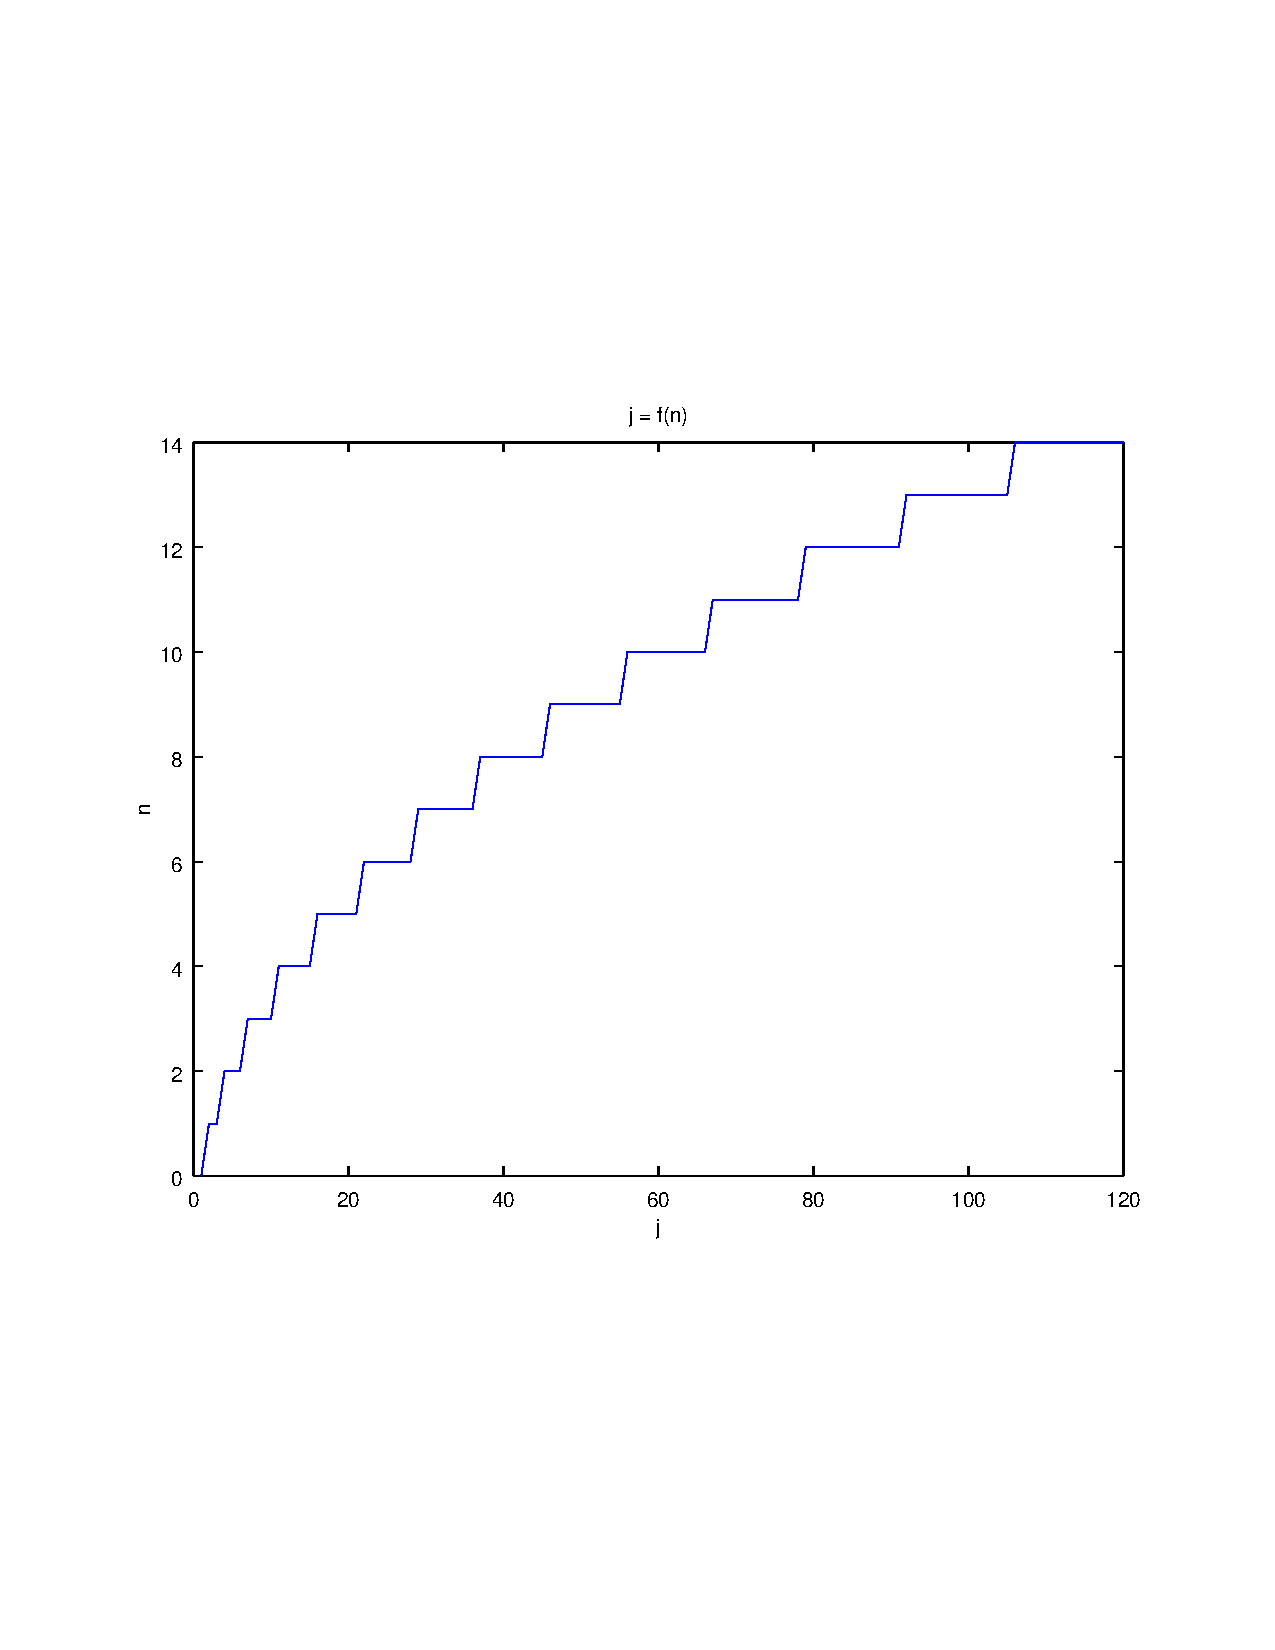
\includegraphics[width=\textwidth]{J_n.pdf}
	\caption{}
\end{figure}


\bibliographystyle{unsrt}
\bibliography{biblio}
\end{document}